
\section{Application à l'adaptation physique}
\label{sec:adapPhysique}

\indent De la même façon que l'adaptation Level Set, l'adaptation physique (i.e., à une variable physique calculée sur le maillage, comme le champs de vitesse de l'écoulement) peut être faite avec les deux formulations de \(\omega\). Pour la première, basée sur la variation de la fonction, on n'a pas de remarques supplémentaires à faire : au contraire de la fonction Level Set, qui est toujours lisse, les variables physiques dans les problèmes de mécanique de fluides qui nous intéressent présentent en général des discontinuités, ayant ainsi des fortes gradients et hessiens qui permettent une bonne adaptation. Alors, il ne faut pas construire une autre fonction à adapter. 

\indent On va ainsi détailler seulement le deuxième calcul de \(\omega\) :

\subsection{Calcul des tailles désirées}

\indent Le calcul des tailles présenté dans la suite s'inspire dans \cite{cecile_these} et \cite{frey_alauzet}, et s'est basée sur la notion de métrique : pour chaque noued \(i\) du maillage, on définit une matrice \(\met_i \ 2 \times 2\) (dans le cas bidimensionnel) qui minimise un estimateur de l'erreur d'interpolation de la solution sur le maillage.

\indent Étant \(\Pi_hu\) l'interpolation de \(u\) sur le maillage, cet estimateur est donné, pour chaque élément \(K\) du maillage, par

\begin{equation}
	\label{eq:erreur_interp}
	||u-\Pi_hu||_{\infty,K} \leq c_d \max_{x \in K}{\max_{\vec{e} \in E_K}{\langle \vec{e}, |H_u(\vecx)| \vec{e} \rangle}}
\end{equation}

\noindent où \(c_d = \frac{2}{9}\) est obtenu avec un développement de Taylor de \eqref{eq:erreur_interp} dans son point de maximum. On veut imposer une  limite \(\epsilon\) à cette erreur : 

\begin{equation*}
	||u-\Pi_hu||_{\infty,K} = \epsilon
\end{equation*}

\indent En définissant la métrique

\begin{equation}
	\label{eq:def_metrique}
	\met = \frac{c_d}{\epsilon}H_u(\vecx)
\end{equation}

\noindent la longueur des arêtes selon cette métrique est alors

\begin{equation*}
	l_{\met_i} = \langle \vec{e}, |\met_i| \vec{e} \rangle = 1
\end{equation*}

\noindent c'est à dire, la métrique qui assure l'erreur d'interpolation désirée est celle telle que le maillage soit unitaire \cite{cecile_these,frey_alauzet}.

\indent Étant la métrique une matrice positive définie symétrique, elle est toujours diagonalisable es ses valeurs propres \(\tilde{\lambda}_i^j, j=1,2\), sont toujours réelles. En effet, la métrique peut être représentée par une ellipse (ou un ellipsoïde, en 3D), dont les vecteurs propres donnent la direction des axes et les valeurs propres sa taille, selon la relation \(h_j =  \frac{1}{\sqrt{\tilde{\lambda}_i^j}}\) \cite{leo}. Ainsi, las caractéristiques géométriques des éléments (taille, forme et orientation) est contenue dans la métrique, et comme on a plus d'un valeur propre, on en définit ainsi des éléments anisotropes.

\indent Néanmoins, on va considérer un cas isotrope, en prenant la plus grande valeur propre de la métrique, ce qui donne la plus petite taille de chaque élément. Enfin, en établissant des seuils minimal et maximal pour la taille désirée (\(\hm\) et \(\hM\)), et en tenant compte de l'équation \eqref{eq:def_metrique}, les tailles désirées sont calculées à partir de

\begin{equation*}
	h_i = \frac{1}{\sqrt{\min\left(\max\left(\frac{c_d}{\epsilon}\lambda_i,\hM^{-2}\right),\hm^{-2}\right)}}
\end{equation*}

\noindent où \(\lambda_i = \max\limits_{j=1,2}{|\lambda_i^j}|\) est la plus grande valeur propre du hessien \(H_u(\vecx_i) \), en valeur absolue.

\indent Également au cas de l'adaptation Level Set, les tailles définies sur le maillage sont lissées avec une gradation de 10\%.

\indent La figure \ref{fig:metPhys} présente un exemple de métrique calculée à partir d'une variable physique .

\begingroup
	\begin{minipage}[t]{.5\linewidth}
		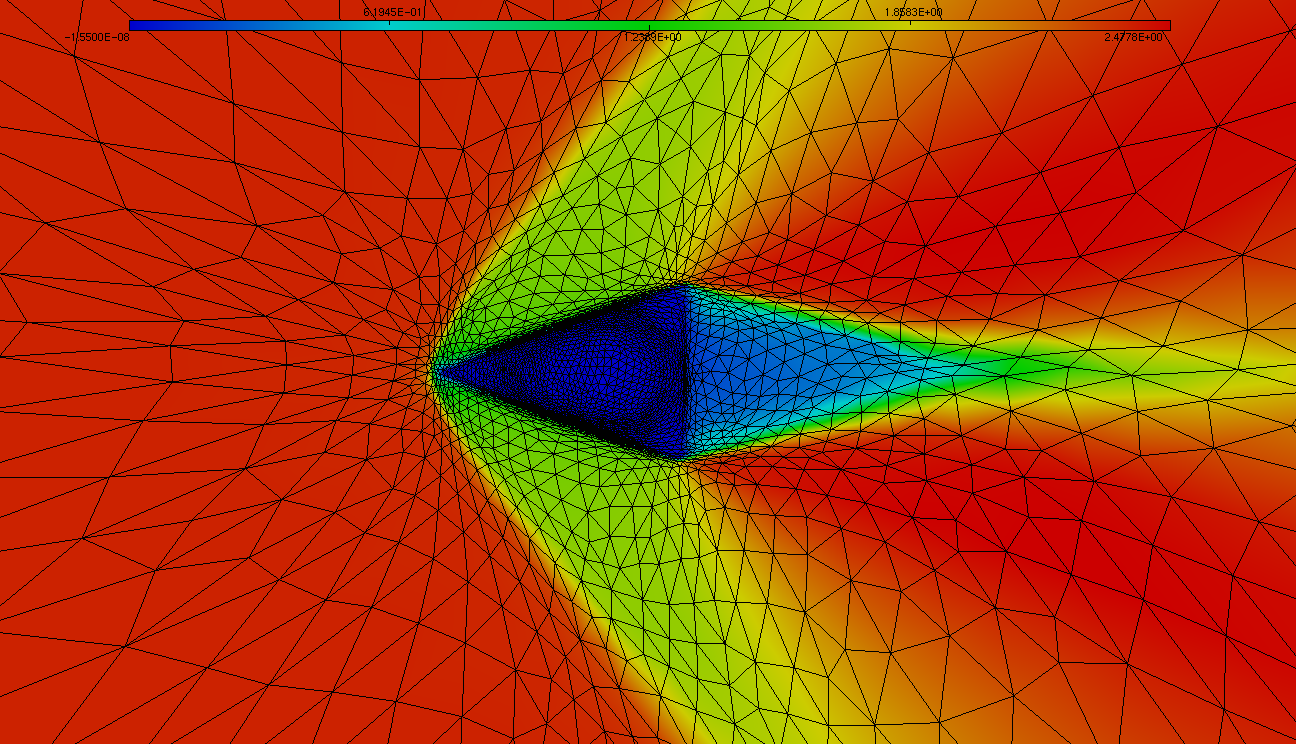
\includegraphics[scale=.15]{Bordeaux/figures/AdapPhysique/u.png}
		\captionof{subfigure}{Composant horizontale de la vitesse}
	\end{minipage}
	\hfill
	\begin{minipage}[t]{.5\linewidth}
		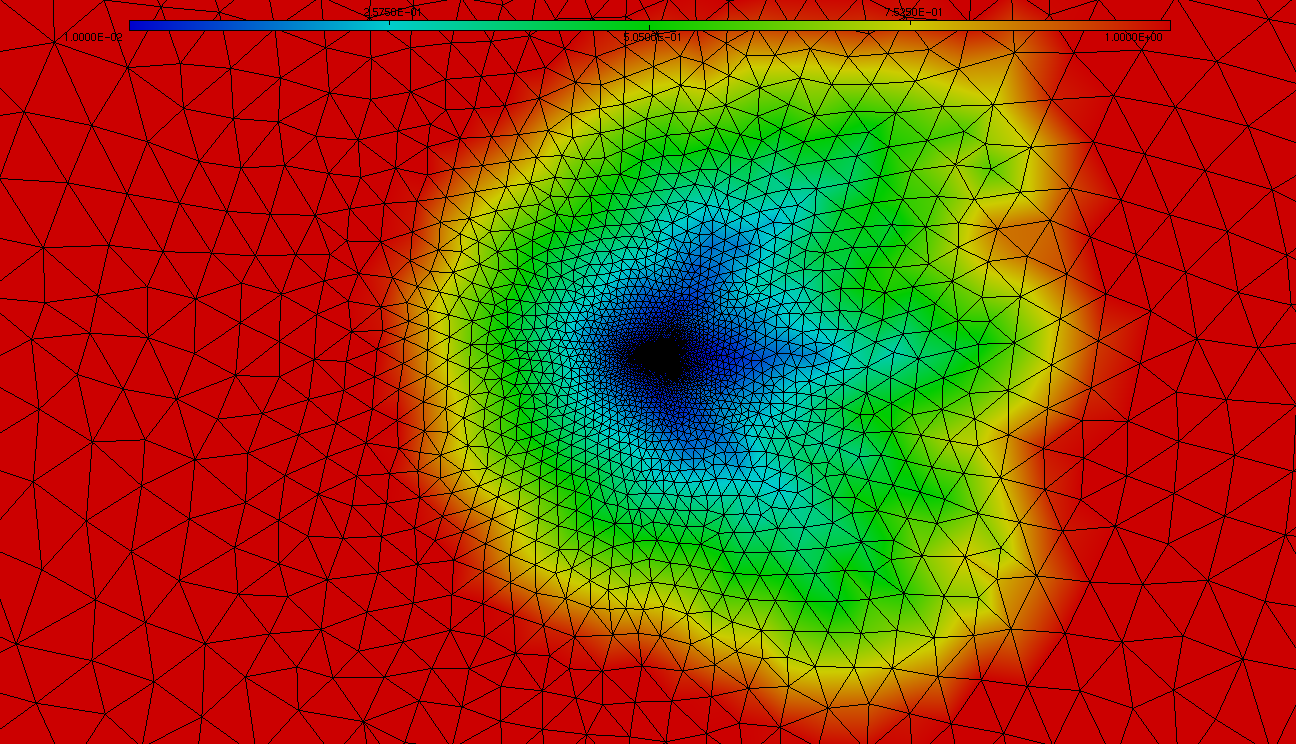
\includegraphics[scale=.15]{Bordeaux/figures/AdapPhysique/met.png}
		\captionof{subfigure}{Tailles calculées à partir de la métrique associée}
	\end{minipage}	
	\captionof{figure}{Écoulement autour d'un triangle - calcul des tailles désirées à partir d'une variable physique \label{fig:metPhys}}
\endgroup

\subsection{Couplage entre adaptation Level Set et adaptation physique}

\indent L'objectif principal de l'ensemble du travail réalisée dans ce projet est l'application du modèle et de la bibliothèque développés à la résolution de problèmes de la mécanique de fluides, afin d'améliorer la précision des résultats. Ainsi, un bon maillage serait adapté au même temps à la surface de l'objet dans le domaine et au profil de la variable physique calculée (la vitesse, par exemple), et par conséquent les deux types de adaptation présentées ci-dessus doivent être considérées.

\indent Pour coupler les deux adaptations, on va intersecter ses respectives métriques : en notant \(h_i^{LS}\) et \(h_i^{phys}\) la taille calculée pour le noeud \(i\) à partir des métriques, respectivement, de la fonction Level Set et de la variable physique (avant le lissage), on choisit le taille

\begin{equation*}
	h_i = \min(h_i^{LS},h_i^{phys})
\end{equation*}

\indent Ensuite, on applique le même lissage avec une gradation de 10\%.

\indent Pour le couplage des deux adaptation, on a proposé la procédure itérative suivante :  

\begin{enumerate}
	\item Calcul de la métrique associée à la fonction Level Set;
	\item Adaptation du maillage à cette métrique;
	\item \label{item:resolution} Résolution du problème physique sur le maillage adapté;
	\item Calcul de la métrique associée à la variable physique et intersection avec la métrique de la fonction Level Set 
	\item Adaptation du maillage à cette métrique, en partant du dernier maillage obtenu, mais toujours avec le même maillage de référence (le maillage de départ, non adapté);
	\item Retour au pas \ref{item:resolution}
\end{enumerate}

\subsection{Résultats}

\indent La procédure décrite ci-dessus a été utilisé dans la résolution d'un flot supersonique 2D autour d'un triangle, avec une méthode de distribution de résidus appliquée aux équations de Navier Stokes pénalisées. Ce cas test est présenté et résolu dans \cite{leo}, dont les paramètres de l'écoulement sont les mêmes utilisés ici.

\indent Étant le modèle pénalisé, le triangle n'est pas discrétisée dans le domaine, ce qui signifie qu'il y a des mailles à son intérieur. En effet, le terme de pénalisation est appliqué exactement aux noeuds à l'intérieur de l'objet, identifiés par la signe de la fonction Level Set. Ainsi, la première adaptation de notre procédure (adaptation à la ligne de niveau 0 de la fonction Level Set) est de grande importance pour la représentation de la surface et la résolution précise des équations dans ses voisinages.

\indent La solution physique utilisée pour les adaptations suivantes est la composante horizontale de la vitesse. 

\indent Les tests ont été réalisées avec l'objectif de vérifier l'évolution de la qualité du résultat dans chaque itération de la procédure. Cette vérification sera faite de façon qualitative et quantitative. Pour la première, on regardera par exemple la régularité du profil de la vitesse et de ses lignes de niveau et la résolution autour des coins du triangle. Pour la deuxième, on adoptera le même critère utilisé par \cite{leo}, en calculant l'angle entre le choc et l'axe \(y=0\), en utilisant un point du choc proche à cet axe, et identifiée par la proximité des lignes de niveau de la vitesse. La résolution analytique du problème fournit un angle \(\beta=53.33^o\), qu'on utilisera pour la comparaison.

\indent Le résultat présenté dans les figures \ref{fig:adapPhysDoms} à \ref{fig:adapPhysPlotB} a été fait sur un domaine circulaire, de rayon vingt fois plus grand que la taille du triangle, afin de représenter un domaine infini, qui minimise l'influence des bords. Afin d'éviter un nombre trop grand de points, mais encore avec un bon raffinement dans les régions les plus proches des bords pour bien capturer le choc, les tailles des éléments ont été définies en fonction de la distance au centre du domaine, augmentant linéairement entre 0.002 et 1. Le résultat est un maillage avec 12664 noeuds et 25200 éléments.

\begingroup
	\begin{minipage}[t]{.5\linewidth}
		\centering
		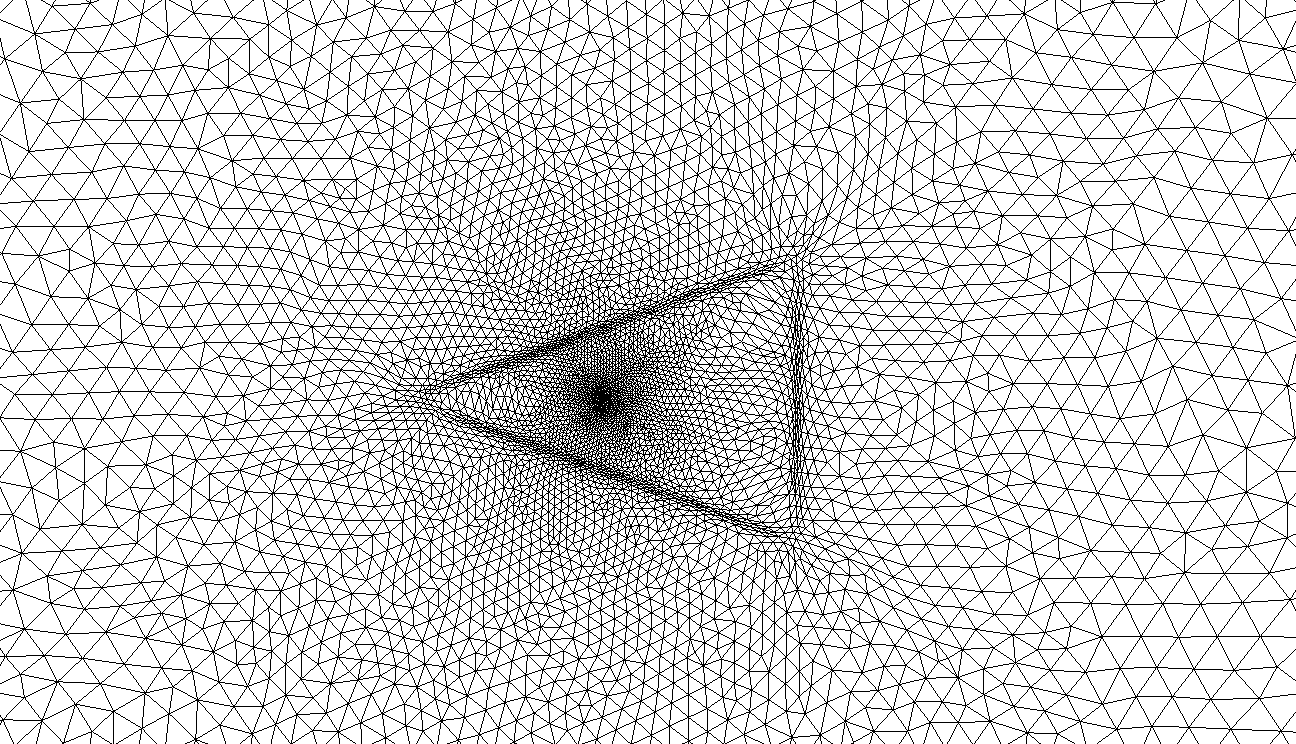
\includegraphics[scale=.15]{Bordeaux/figures/AdapPhysique/dom4bI0.png}
		\captionof{subfigure}{Première adaptation}
	\end{minipage}
	\hfill
	\begin{minipage}[t]{.5\linewidth}
		\centering
		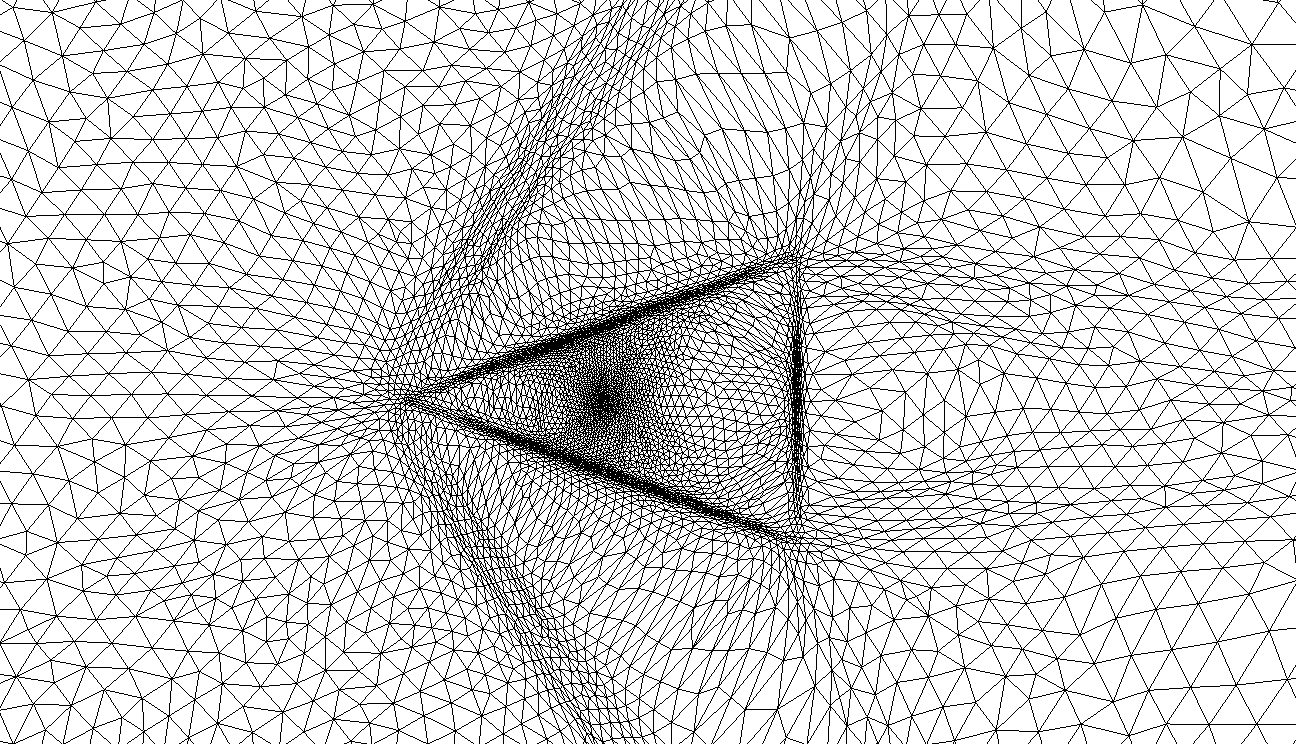
\includegraphics[scale=.15]{Bordeaux/figures/AdapPhysique/dom4bI1.png}
		\captionof{subfigure}{Deuxième adaptation}
	\end{minipage}
	\begin{minipage}[t]{1.\linewidth}
		\centering
		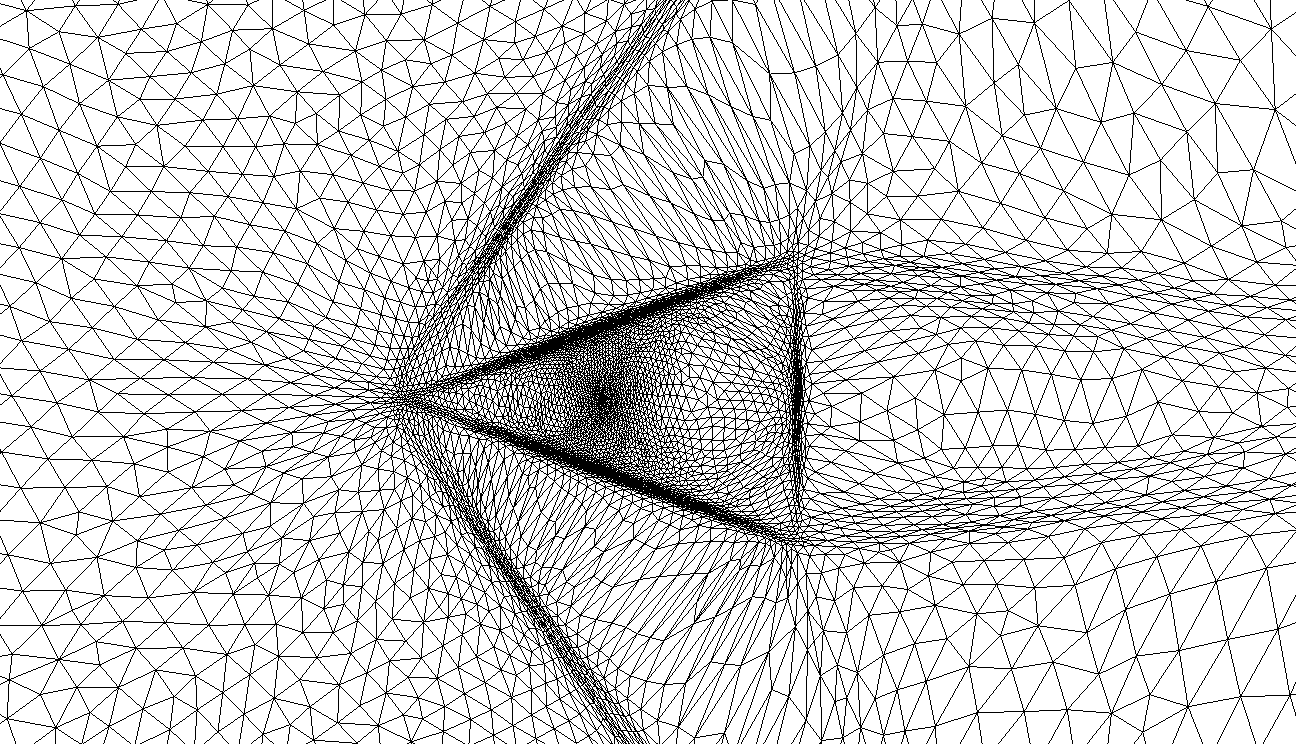
\includegraphics[scale=.15]{Bordeaux/figures/AdapPhysique/dom4bI2.png}
		\captionof{subfigure}{Troisième adaptation}
	\end{minipage}
	\captionof{figure}{Séquence de maillages adaptés obtenus \label{fig:adapPhysDoms}}
\endgroup

\begingroup
	\begin{minipage}[t]{.5\linewidth}
		\centering
		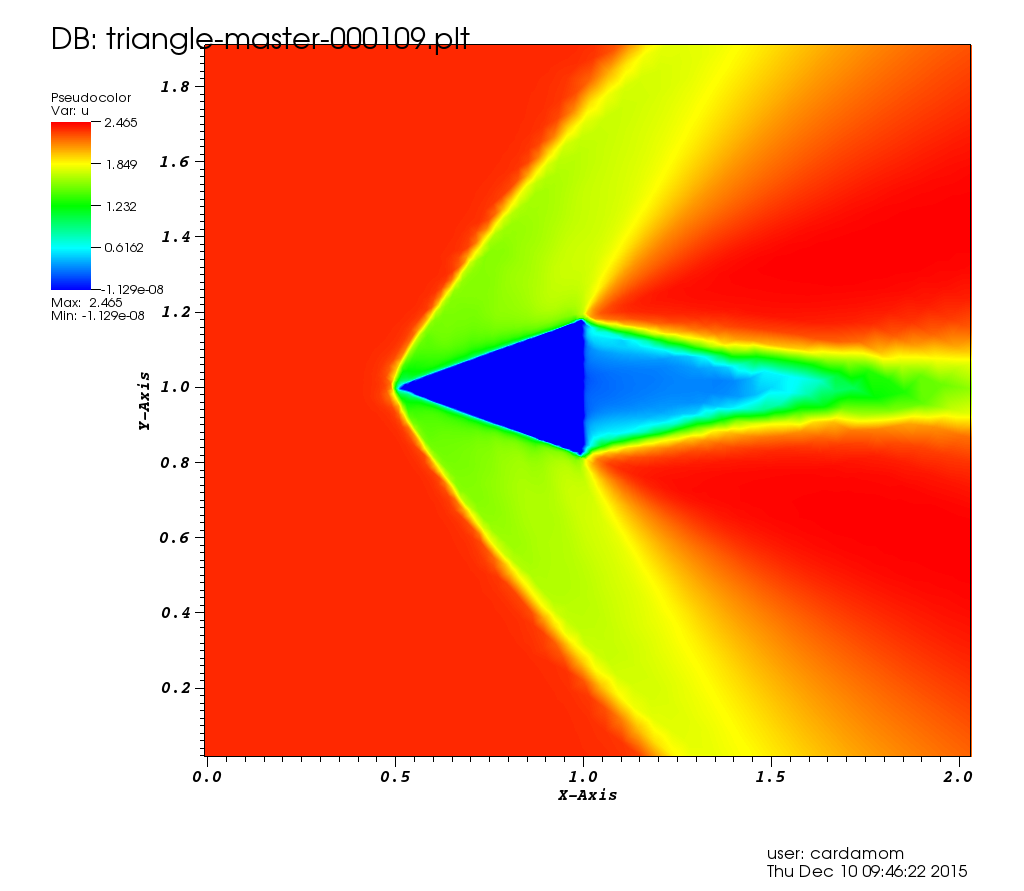
\includegraphics[scale=.2]{Bordeaux/figures/AdapPhysique/Plot4bI0A.png}
		\captionof{subfigure}{Première résolution}
	\end{minipage}
	\hfill
	\begin{minipage}[t]{.5\linewidth}
		\centering
		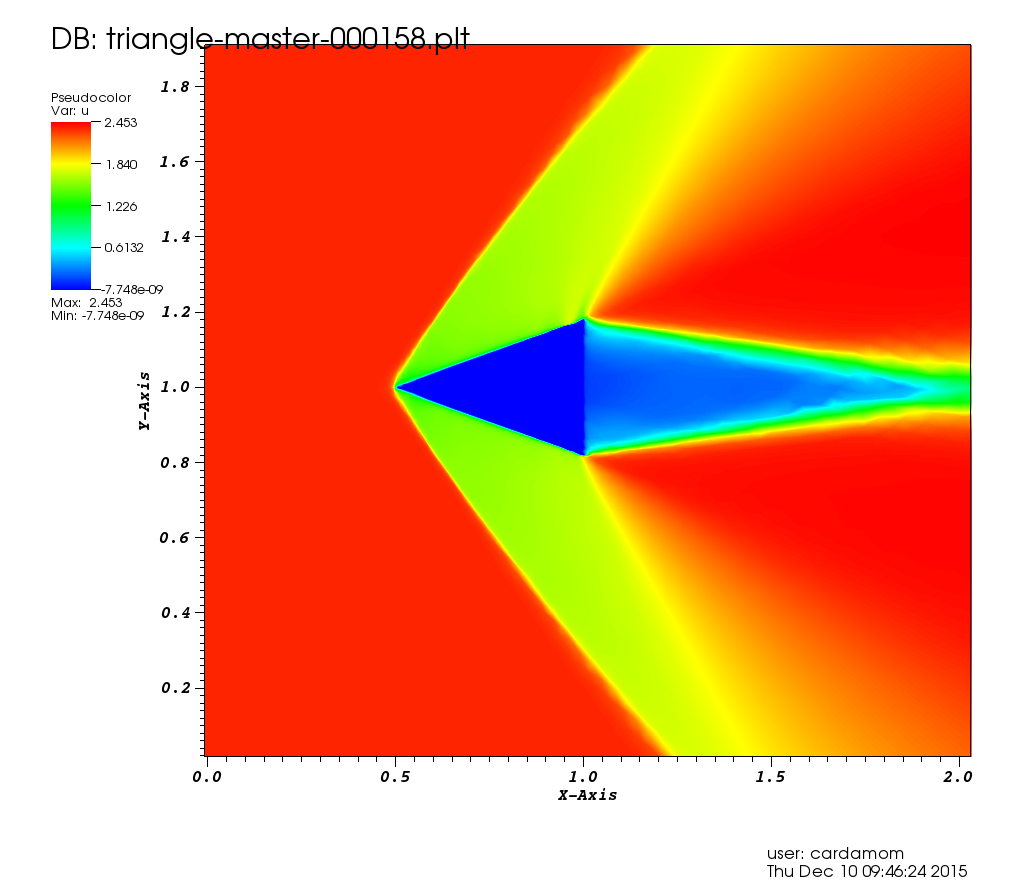
\includegraphics[scale=.2]{Bordeaux/figures/AdapPhysique/Plot4bI1A.png}
		\captionof{subfigure}{Deuxième résolution}
	\end{minipage}
	\begin{minipage}[t]{1.\linewidth}
		\centering
		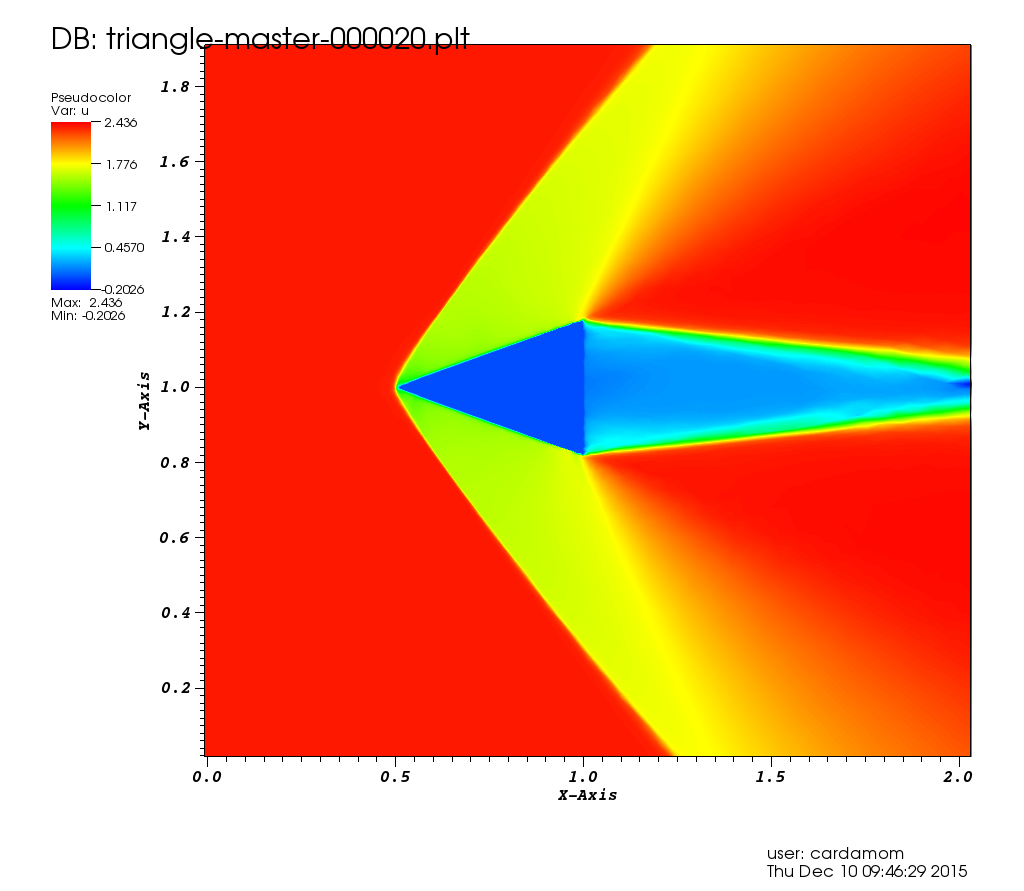
\includegraphics[scale=.2]{Bordeaux/figures/AdapPhysique/Plot4bI2A.png}
		\captionof{subfigure}{Troisième résolution}
	\end{minipage}
	\captionof{figure}{Composante horizontale de la vitesse \label{fig:adapPhysPlotA}}
\endgroup

\begingroup
	\begin{minipage}[t]{.5\linewidth}
		\centering
		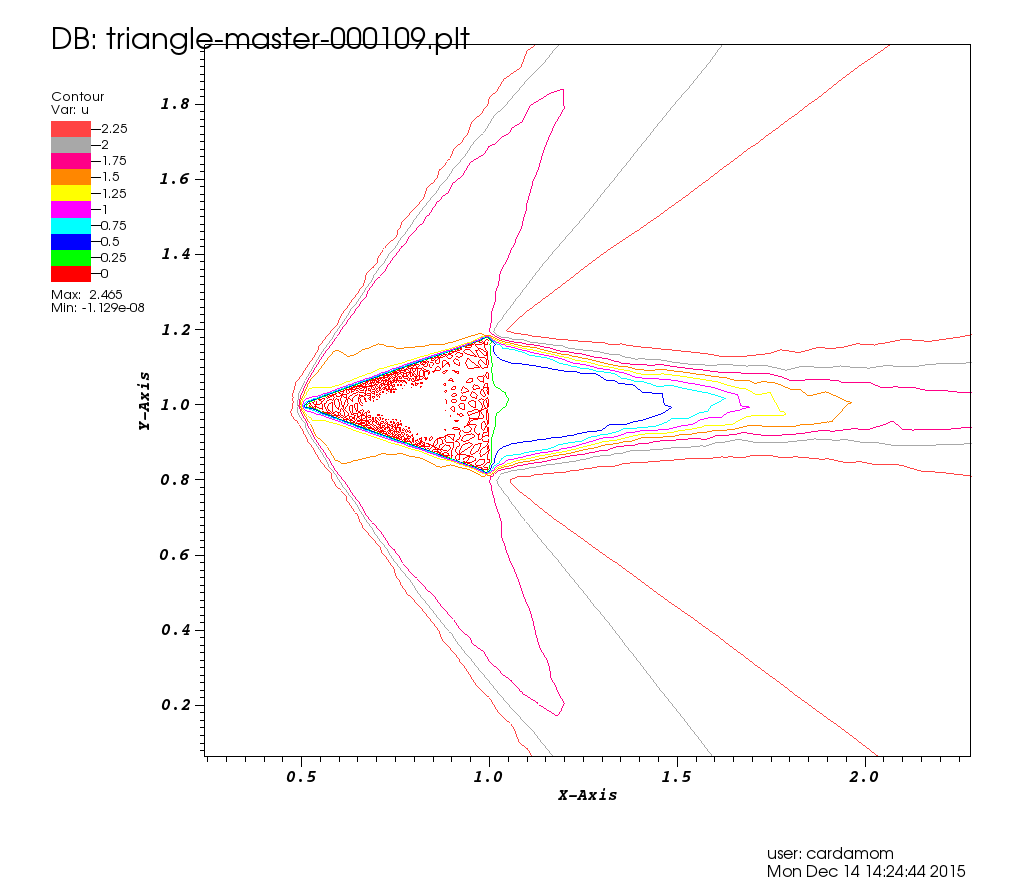
\includegraphics[scale=.2]{Bordeaux/figures/AdapPhysique/Contour4bI0.png}
		\captionof{subfigure}{Première résolution}
	\end{minipage}
	\hfill
	\begin{minipage}[t]{.5\linewidth}
		\centering
		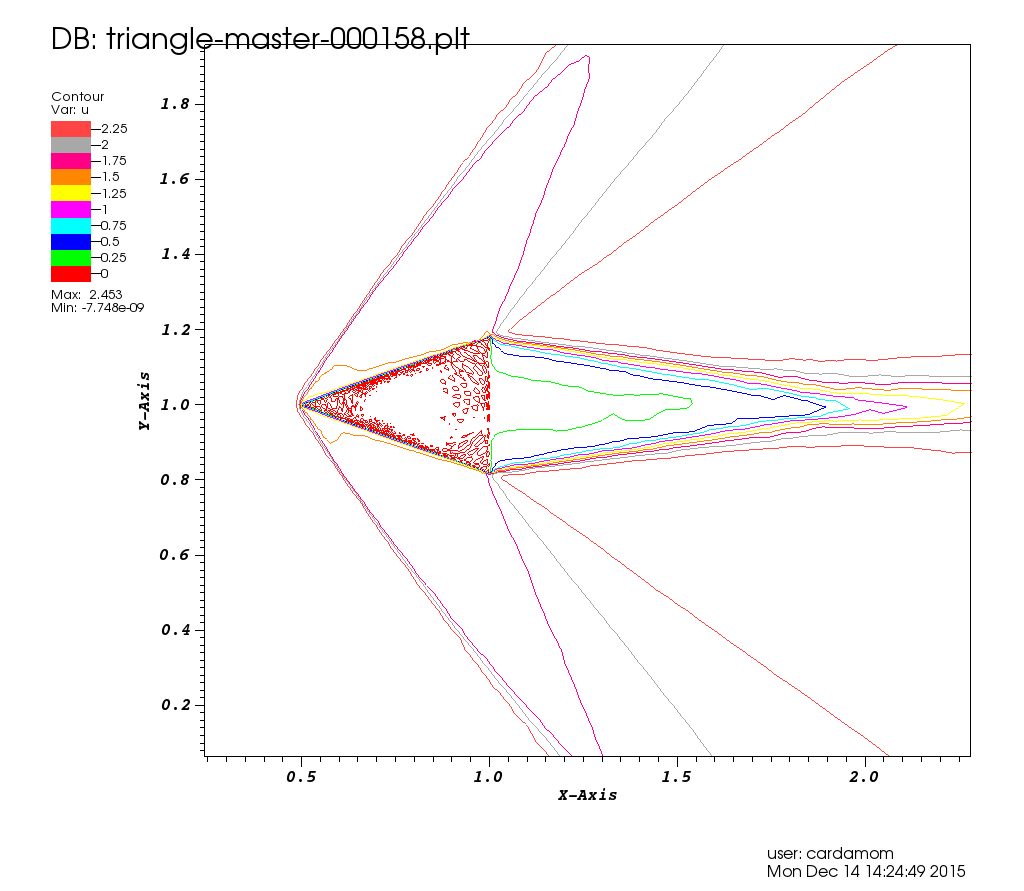
\includegraphics[scale=.2]{Bordeaux/figures/AdapPhysique/Contour4bI1.png}
		\captionof{subfigure}{Deuxième résolution}
	\end{minipage}
	\begin{minipage}[t]{1.\linewidth}
		\centering
		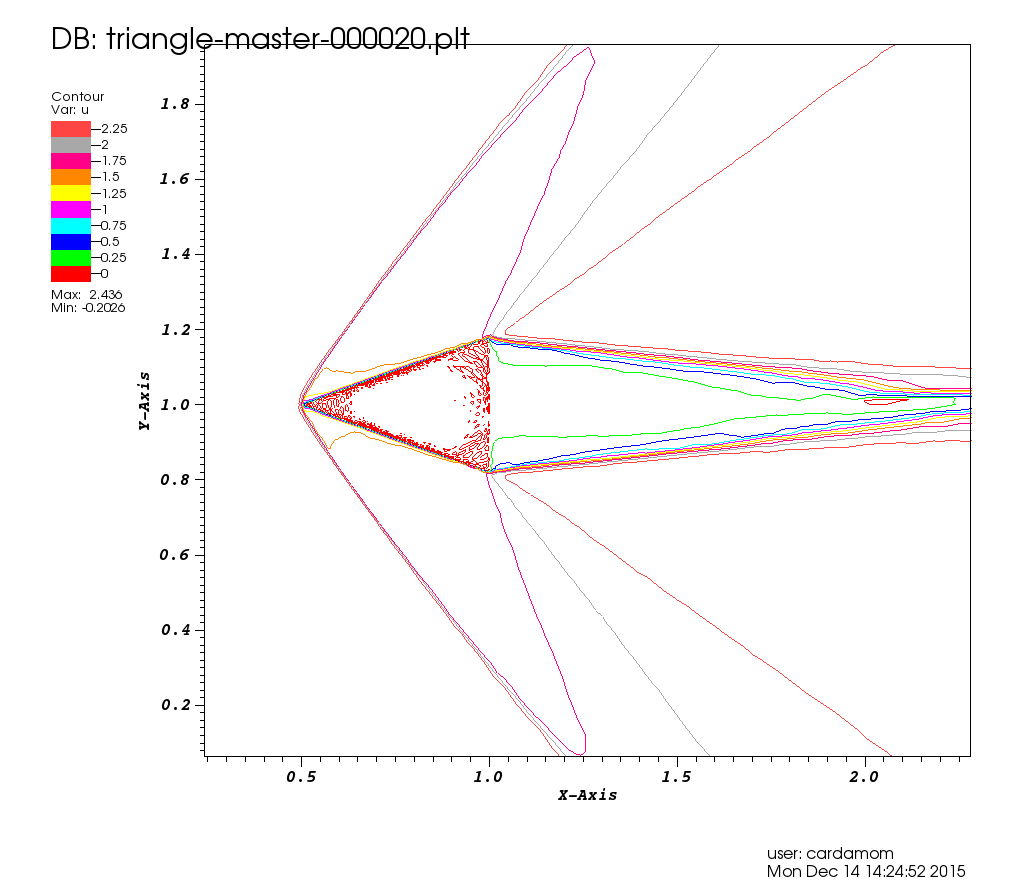
\includegraphics[scale=.2]{Bordeaux/figures/AdapPhysique/Contour4bI2.png}
		\captionof{subfigure}{Troisième résolution}
	\end{minipage}
	\captionof{figure}{Lignes de niveau de la composante horizontale de la vitesse \label{fig:adapPhysContour}}
\endgroup

\begingroup
	\begin{minipage}[t]{.5\linewidth}
		\centering
		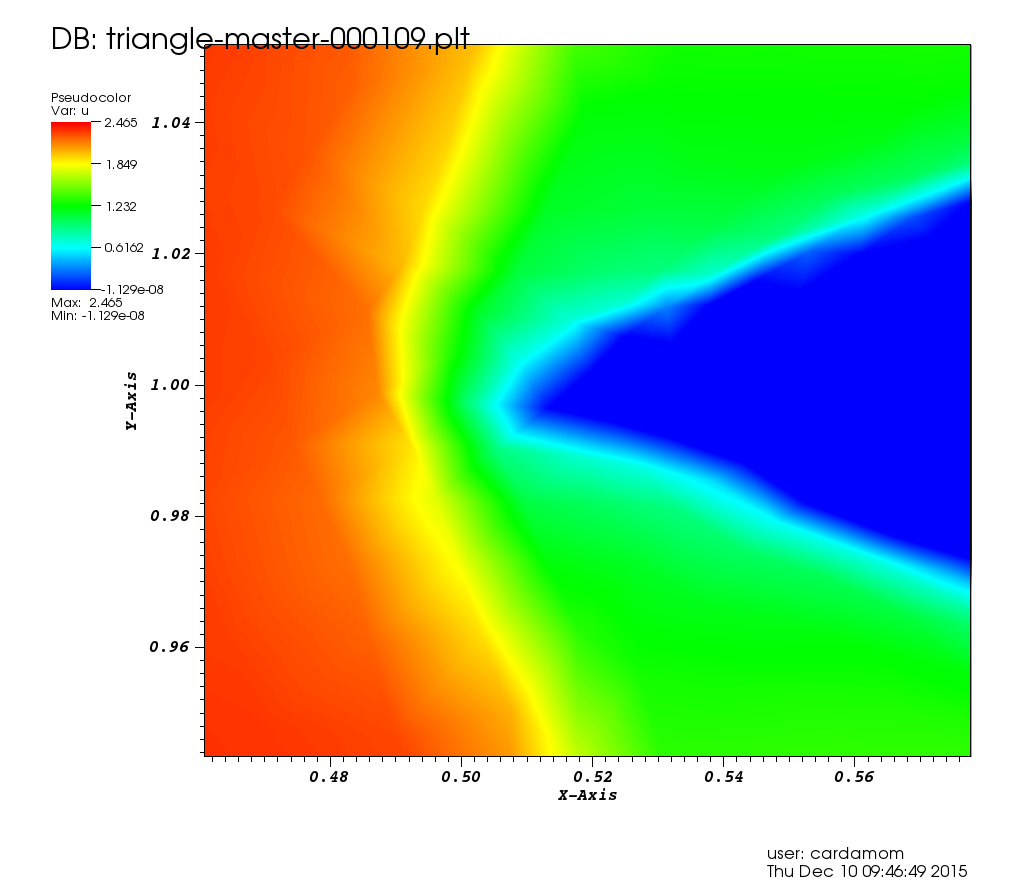
\includegraphics[scale=.2]{Bordeaux/figures/AdapPhysique/Plot4bI0B.png}
		\captionof{subfigure}{Première résolution}
	\end{minipage}
	\begin{minipage}[t]{.5\linewidth}
		\centering
		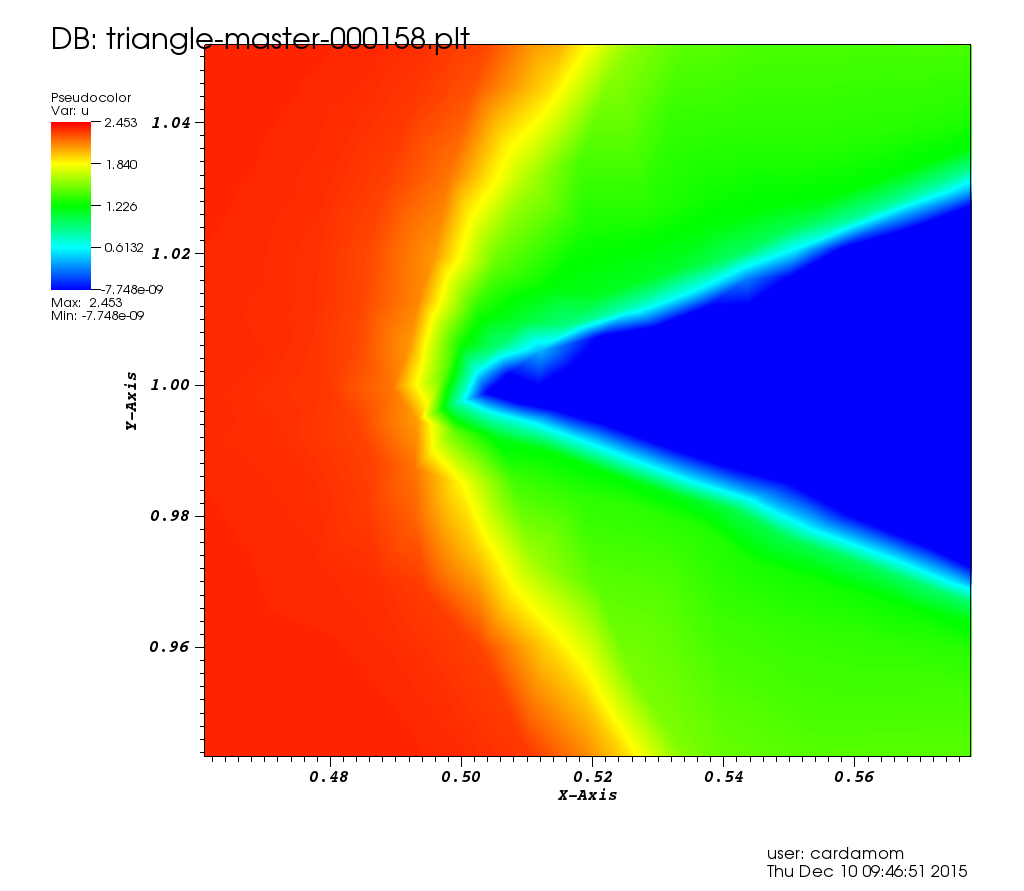
\includegraphics[scale=.2]{Bordeaux/figures/AdapPhysique/Plot4bI1B.png}
		\captionof{subfigure}{Deuxième résolution}
	\end{minipage}
	\begin{minipage}[t]{1.\linewidth}
		\centering
		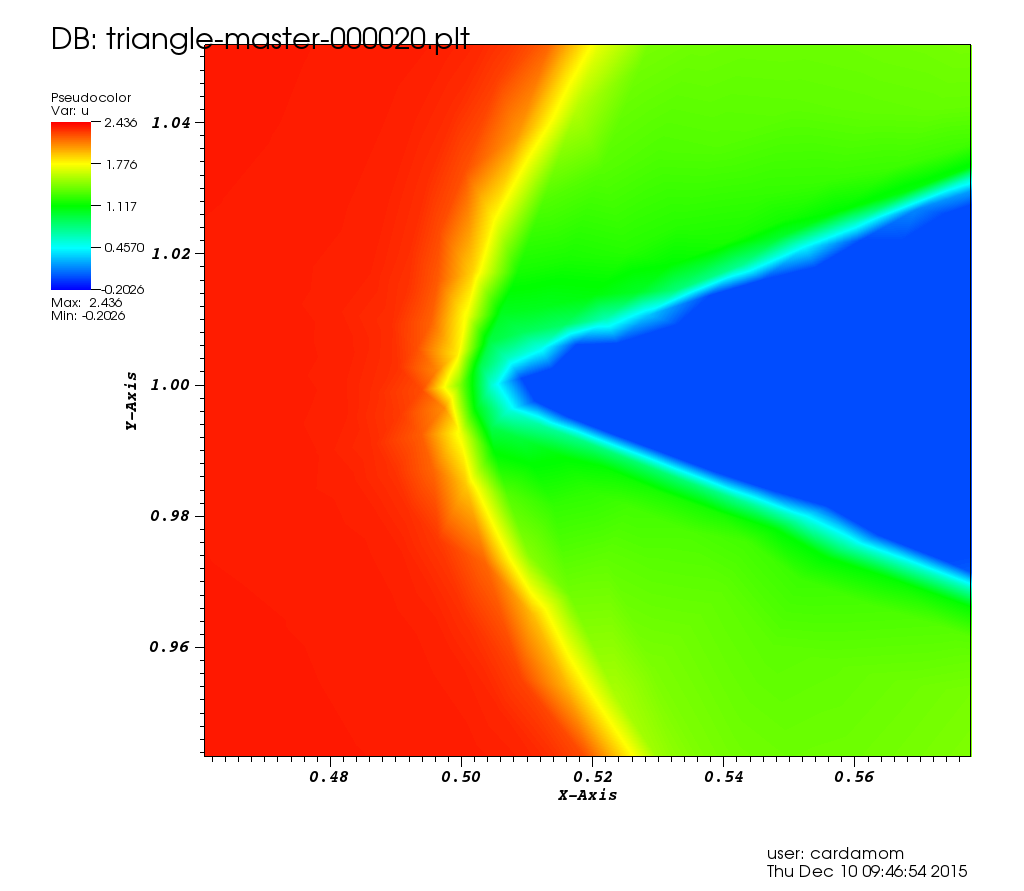
\includegraphics[scale=.2]{Bordeaux/figures/AdapPhysique/Plot4bI2B.png}
		\captionof{subfigure}{Troisième résolution}
	\end{minipage}
	\captionof{figure}{Détail - Composante horizontale de la vitesse \label{fig:adapPhysPlotB}}
\endgroup

\indent L'angle \(\beta\) a évolué selon les valeurs présentées dans le tableau \ref{tab:beta}

\begin{table}[!ht]
	\centering
	\begin{tabular}{c|c}
		Résolution & \(\beta\) \\
		\hline
		1 & \(55.68^\circ\) \\
		2 & \(53.92^\circ\) \\
		3 & \(53.01^\circ\) \\
	\end{tabular}
	\caption{Angle entre le choc et l'axe \(y=0\) \label{tab:beta}}
\end{table}

\indent Ces résultats montrent que la procédure proposée permet en effet d'améliorer la résolution du problème physique : à chaque itération, le champ de vitesse calculée devient mieux définie, avec des lignes de niveau plus régulières, et l'angle entre le choc et l'axe \(y=0\) s'approche de la valeur analytique. Néanmoins, quelques difficultés sont encore présentes dans las tests réalisées, notamment la génération de maillages permettant un calcul stable (considérant les fortes discontinuités qui caractérisent ce cas test) et le fait que, comme montre la figure \ref{fig:adapPhysPlotB}, le choc n'est pas attaché au triangle, au contraire du résultat théorique, ce qui s'explique par les limitations du raffinement du maillage.